%! TEX root = **/010-main.tex
% vim: spell spelllang=en:

\section{Description of pre-processing of data}%
\label{sec:desc-prep}

% Kind of preprocessing done to the original data:  Have you simplified the dataset?
% Removed some examples?
% Feature selection done?
% Did you enrich your dataset with other columns or more information?
% Imputing/removing missing values? 
% Simplification of values? 
% Normalization? 
% Remember that you should describe the all procedures performed on your raw dataset.

\subsection{Feature Removal}

Initially, we removed all of the variables which didn't provide any useful information
such as names and identification numbers: \texttt{kepid}, \texttt{rowid}, 
\texttt{kepoi\_name}, \texttt{kepler\_name} or \texttt{koi\_tce\_delivname}.

Next, we investigated the presence of missing data in the dataset, and we found that three
variables were mostly missing. Specially \texttt{koi\_teq\_err1} and 
\texttt{koi\_teq\_err2}, which represent the positive and negative error 
of \texttt{koi\_teq} respectively, are completely missing. Therefore, we proceeded to 
remove them as they didn't provide any information whatsoever. How we treated the rest
of the missing values will be explained in an upcoming section.

We also removed four features that were flags representing whether the exoplanet
measurements had passed some tests. Since this flags directly impact the
target feature, as \texttt{koi\_disposition} will be FALSE NEGATIVE when it fails
at least one of the tests and CONFIRMED when it passes all the tests and is confirmed,
and are calculated using the raw data thus simplifying the problem. Furthermore, the
main objective of this classification problem is to work directly with the raw Kepler
measurements and not with processed data such as these flags.

Furthermore, there are two other columns, \texttt{koi\_pdisposition} and 
\texttt{koi\_score},
that we decided to erase as well, as 
\texttt{koi\_pdisposition} represents the predicted \texttt{koi\_disposition}
(our target) and \texttt{koi\_score} illustrates the level of confidence of
that prediction, based on the aforementioned flags. Hence, they are directly
linked to our target as well. As a matter of fact, in close to 70\% of the
7316 remaining examples the \texttt{koi\_disposition} and \texttt{koi\_pdisposition}
have the same value.

\subsection{Example Removal}

As explained in the description of the original dataset, we decided to remove all 
examples that had \texttt{koi\_dispoistion} equal to CANDIDATE, as we want to
train and validate our models using exoplanets that we know for sure whether
they are or aren't confirmed, and not with examples that are pending for validation.
This resulted in the elimination of 2248 entries out of the original 9564, 
leaving us with 7316 examples.

\subsection{Value Transformation}

Because some algorithms only work with numerical features, we had to transform our
target column from categorical to numerical. Since we had removed all instances of
CANDIDATE, there were no examples of NOT DISPOSITIONED and the categories don't follow
a particular order, we opted for One-Hot encoding. Furthermore, as we only had two
categories, we didn't need to create extra columns, we simply transformed the existing
\texttt{koi\_disposition} column to be 1 when the example is CONFIRMED and 0 when
it isn't, meaning it is a FALSE POSITIVE.

\subsection{Error Treatment}

We scanned our dataset looking for errors and we weren't able to find any. We checked
that numerical values were within the plausible ranges, like for example that the
planet radius or temperatures were positive. We also verified that all categorical 
features only contained the expected categories.

\subsection{Missing Data Treatment}

For the remaining missing data, we decided to fill those empty cells with the mean
of the feature. We were able to do that because all of our columns with missing values
were of numerical type.

\subsection{Feature Selection}%
\label{sub:feature_removal}

The next step in our pre-processing script, consists in reducing the number of features
by selecting the ones that provide the best results. To do that, we first need to
standardize the data, by transforming all variables so they have a mean equal to 0
and standard deviation to 1.

Then, we loop through all possible number of features to be selected, 
excluding the target, that is from 0
to 36, the number of remaining features, and do cross validation using Knn, saving
the average score for each number of selected features. \Cref{fig:feature_cross}
below, shows the results that we obtained. As we can see, we obtained the best score
when only using 25 out of the 36 features.

\begin{figure}[H]
    \centering
    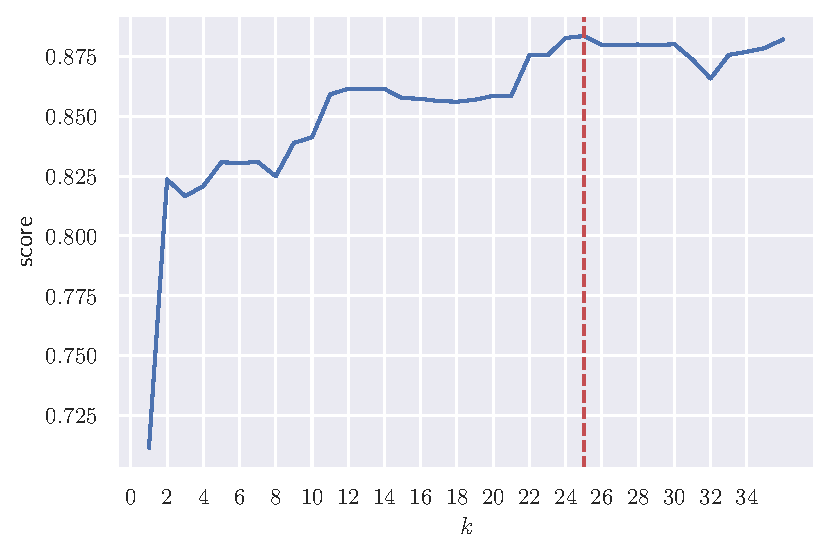
\includegraphics[width=0.6\linewidth]{kbest}
    \caption{Cross validation score for different $k$ values}%
    \label{fig:feature_cross}
\end{figure}

Once we knew that using the best 25 variables provided the best scores, we selected
those 25 columns, which we can see below in \cref{tab:features}.

\begin{table}[H]
    \centering
    \caption{Selected features (25)}%
    \label{tab:features}
    \begin{tabular}{rlc}
\toprule
                   &  Variable &     Score \\
\midrule
1  &     \texttt{koi\_steff\_err1} &  0.193758 \\
2  &            \texttt{koi\_prad} &  0.184690 \\
3  &     \texttt{koi\_steff\_err2} &  0.170011 \\
4  &      \texttt{koi\_prad\_err1} &  0.164256 \\
5  &  \texttt{koi\_duration\_err2} &  0.156999 \\
6  &      \texttt{koi\_prad\_err2} &  0.154296 \\
7  &  \texttt{koi\_duration\_err1} &  0.153266 \\
8  &      \texttt{koi\_model\_snr} &  0.142149 \\
9  &      \texttt{koi\_srad\_err1} &  0.132922 \\
10 &   \texttt{koi\_time0bk\_err1} &  0.131132 \\
11 &          \texttt{koi\_period} &  0.128600 \\
12 &     \texttt{koi\_slogg\_err2} &  0.123361 \\
13 &   \texttt{koi\_time0bk\_err2} &  0.123268 \\
\bottomrule
\end{tabular}
\quad
\begin{tabular}{rlc}
\toprule
                   &  Variable &     Score \\
\midrule
14 &    \texttt{koi\_slogg\_err1} &  0.120881 \\
15 &          \texttt{koi\_steff} &  0.115671 \\
16 &   \texttt{koi\_period\_err2} &  0.109981 \\
17 &   \texttt{koi\_period\_err1} &  0.108709 \\
18 &    \texttt{koi\_insol\_err2} &  0.108357 \\
19 &          \texttt{koi\_depth} &  0.106608 \\
20 &    \texttt{koi\_insol\_err1} &  0.105152 \\
21 &           \texttt{koi\_srad} &  0.102525 \\
22 &          \texttt{koi\_insol} &  0.102372 \\
23 &            \texttt{koi\_teq} &  0.100868 \\
24 &         \texttt{koi\_impact} &  0.099700 \\
25 &                 \texttt{dec} &  0.099228 \\
\, & & \\
\bottomrule
\end{tabular}

\end{table}

Therefore, our dataset for the rest of the project consists of the above variables
together with our target column \texttt{koi\_disposition}.

\subsection{Sampling}

Finally, because we still have 7316 examples, we decided to do reduce the size of the
dataset to 2000 entries through sampling. We did it mainly due to performance issues,
to make the dataset more manageable and reduce execution times. We also checked that
the resulting sampled dataset respected the proportions of our
target column, and we obtained a very similar one.